%\begin{savequote}[6cm]
%<< Some other great quote  >>
%\qauthor{Someone}
%\end{savequote}
\chapter{État de l'art}\label{chap:rw}
\chaptertoc


\begin{figure}[ht]
  \centering
  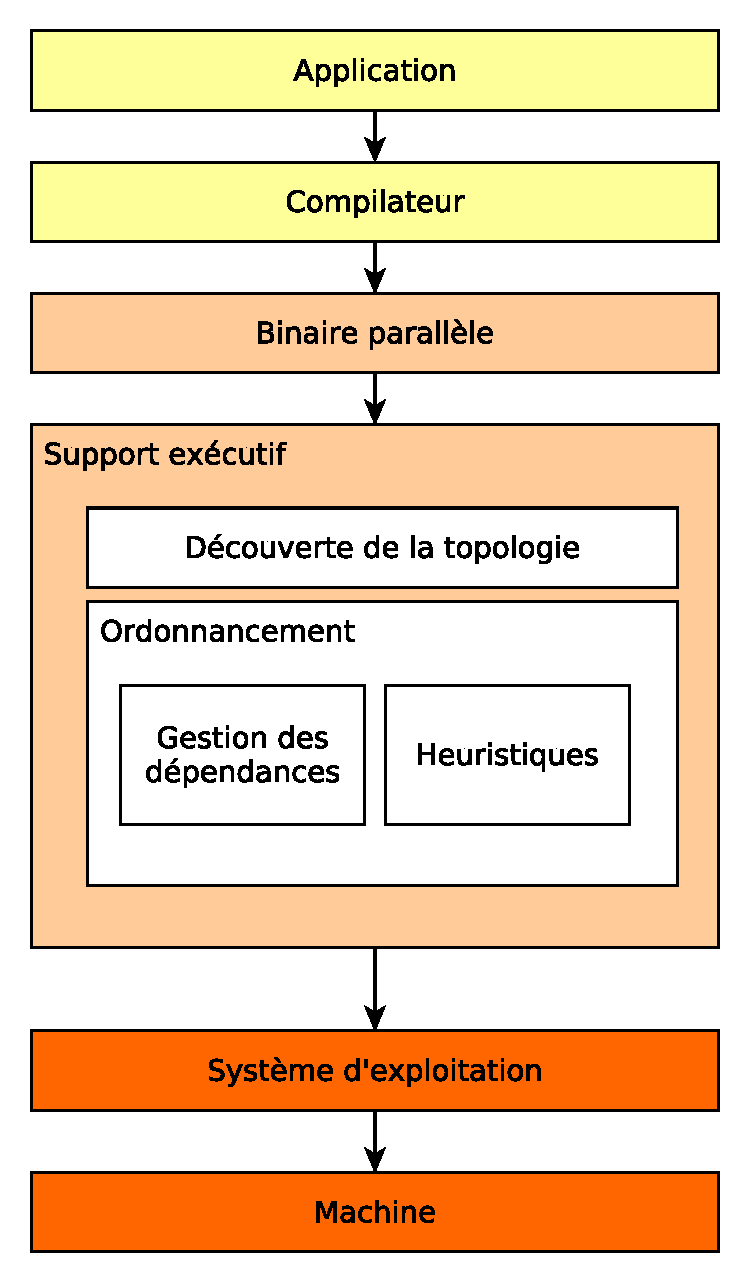
\includegraphics[width=0.5\textwidth]{schema-application-os}
  \caption{Schéma des acteurs impliqués dans l'exécution d'une application}\label{fig:rw:application-os}
\end{figure}

L'objectif de ce chapitre est de donner un aperçu des travaux existants dans le contexte de cette thèse.
Comme on peut le voir sur la figure~\ref{fig:rw:application-os}, un certain nombres d'acteurs sont impliqués dans l'exécution d'une application.

Les parties application, système d'exploitation, et matériel ont été traitées dans le chapitre précédent~; ce chapitre ce concentrera dans un premier temps sur une partie précise des supports exécutifs, en abordant les différentes techniques d'ordonnancement présentes dans l'état de l'art pour cibler spécifiquement les machines NUMA, puis nous regarderons en détails certains supports exécutifs existant, et enfin nous ferons un point sur les compilateurs OpenMP.






\section{Shared memory architectures}\label{sec:context:numa}



\subsection{Single node design}

Talk about cache hierarchy, maybe give some number and a drawing of how it looks like?

\subsection{Interconnecting nodes}

Talk about how nodes are interconnected with each other, give some numbers (?) and some drawing.

\section{Supports exécutifs}\label{sec:rw:other-runtimes}

Il existe un certain nombres d'autres supports exécutifs, pour OpenMP comme d'autres modèle de programmation.
Les sections ci après introduisent ceux ayant des thématiques très proches de cette thèse.

\subsection{XKaapi}

XKaapi~\cite{Gautier2007} est un support exécutif, à base de tâche avec dépendances, ciblant les architectures multicœurs et hétérogènes.
Il repose sur hwloc pour découvrir la topologie de la machine, et utilise ces informations à de multiples endroits.

XKaapi dispose d'un nombre important de fonctionnalités spécifiques à l'ordonnancement de tâches.
Une attention particulière a été portée au coût de création des tâches au sein du support exécutif, qui a été diminué au maximum (TODO : ref needed).
Le moteur d'ordonnancement de XKaapi fonctionne par vol de travail, et implémente les étapes critiques de \emph{sélection} et de \emph{placement} décrites dans la section~\ref{sec:context:runtimes:ws}. Il est facile d'ajouter des heuristiques additionnelles pour ces deux étapes, ce qui nous a permis d'implémenter dans ce support exécutifs les extensions décrites dans la section~\ref{sec:contrib:ws:heuristics}.

Le nombre de files de tâches repose sur les informations fournies par hwloc~: XKaapi implémente une file de tâches par niveau de la hiérarchie (i.e.~: une file par cœur, une file par nœud NUMA, etc...), qui sont éventuellement utilisées par les heuristiques.

Pour la gestion de ces files, XKaapi implémente le protocole THE~\cite{cilk5} proposé par Cilk. Ce protocole permet de faire de manière non bloquante des accès concurrent à la même file de tâche. Le principe est le suivant~: le \emph{voleur} - distant - va venir prendre des tâches en tête de file, et la \emph{victime} (ou le thread local) va venir ajouter ou retirer des tâches en queue de file.
Le seul conflit se produit lorsque la file n'a qu'un seul élément, et il peut être résolu par un simple \emph{compare-and-swap}, se traduisant par un échec de la requête pour l'un, et un succès pour l'autre.

En plus de l'utilisation de ce protocole, XKaapi peut effectuer de l'agrégation de requêtes de vols~: lorsque plusieurs voleur font effectuer des requêtes sur la même victime, seul le premier voleur arrivé va effectuer la requête de vol, et récupérer suffisamment de tâche pour l'ensemble des voleurs.
Les gains théoriques liés à ce mécanismes ont été étudiés par Tchiboukdjian et al.~\cite{Tchiboukdjian2010a}.

Pour observer le comportement des applications exécutées, il dispose d'un outil de génération de traces.
Cela permet une analyse pointue du comportement de l'application, à travers les compteurs de performances matériels et une analyse par type de tâche.
Cet outil nous a permis de faire des observations préliminaires déjà très poussées, sur une étude de cas abordée dans la section~\ref{sec:contribs:apps:cholesky:observations}.

XKaapi est principalement utilisé comme prototype de recherche, et a été utilisé pour l'implémentation de certains travaux proches des thématiques de cette thèse, en particulier celle de la localité des données~\cite{Durand2013, Bleuse2014, Lima2015}.

Enfin il dispose d'une couche de compatibilité pour OpenMP, nommée libKOMP~\cite{Broquedis2012}.
Cette couche implémente à la fois les ABIs de libGOMP et libOMP, ce qui permet de l'utiliser pour exécuter des programmes OpenMP~4.5 directement en compilant via GCC ou Clang, et en changeant le support exécutif chargé à l'exécution.



\subsection{libGOMP}

libGOMP~\cite{Novillo2006} est le support exécutif OpenMP fourni avec le compilateur GCC.

Au niveau des fonctionnalités, il implémente la totalité du standard OpenMP~4.5.
Comme la majorité des supports exécutifs, libGOMP réutilise les threads qui sont créés entre différentes région parallèles successives, pour éviter d'avoir à payer le coût de destruction/création d'un thread inutilement.
Les gestion des constructions à base de boucles et de tâches sont complètement séparées dans le support exécutif.
Vis à vis de la hiérarchie de l'architecture cible, il n'y a aucune disposition particulière pour essayer de la prendre en compte.

Pour la gestion des tâches, il a des différences majeures dans la manière de fonctionner par rapport à XKaapi~: il fonctionne bien par vol de travail, mais en revanche il n'y a qu'une seule file de tâches par \emph{team}, et donc une seule file pour l'ensemble des threads !
Si fonctionnellemment cette caractéristiques n'est pas un problème, cela peut avoir un impact sur les performances compte tenu du fait que tous les threads devront se synchroniser pour accéder à la même struture de données.
Cela se voit d'ailleurs sur la figure~\ref{fig:context:granularity} illustrant l'impact de la granularité des tâches~: pour des petites tailles de bloc (et donc un grand nombre de tâches), libGOMP est loin derrière à cause du surcout entrainé par la gestion de la liste de tâches.
(cf figure 2.4 sur la granularité)

Néanmoins, en tant que support exécutif grand public et largement utilisé, il constitue une référence intéressante.

\subsection{libOMP}

libOMP est le support exécutif OpenMP fourni avec le compilateur Clang, directement basé sur le support exécutif d'Intel fourni avec ICC.
Ils partagent donc exactement les même caractéristiques.

Compte tenu du fait qu'il a été développé à la base par des développeurs d'Intel, une partie de ses fonctionnalités ont été motivées par l'exploitation du matériel produit par Intel comme le Xeon Phi.

De manière similaire à libGOMP, la gestion des boucles et des tâches est séparée, et les threads (et même les \emph{teams} et leurs structures de données associées) sont réutilisés par les régions parallèles successives.

En revanche libOMP se distingue de libGOMP de part ses structures de données~: chaque thread d'une \emph{team} possède une file de tâche propre.
Il conserve donc un fonctionnement très proche de XKaapi, dans le sens où il passe par des fonctions de \emph{sélection} et \emph{placement} lors du vol de travail.
Les heuristiques de base pour ces fonctions sont les suivantes~: la sélection a lieu aléatoirement parmi les file de tâches disponibles~; lors de vols successifs, le voleur essaye en priorité la dernière file dans laquelle il a réussi à voler une tâche. Le placement a lieu dans la file du thread courant.

Bien que ce mécanisme n'ait pas été initialement conçu pour permettre d'interchanger des stratégies, cela proposait une base suffisamment solide pour accueillir les extensions que nous proposons dans le chapitre~\ref{chap:contrib:openmp}.
Les modifications que nous avons apporté à ce support exécutif sont détaillées dans la section~\ref{sec:contribs:perf_eval:libkomp}.


\subsection{OmpSs}\label{subsec:rw:ompss}

OmpSs~\cite{OMPSs} est un modèle de programmation visant à étendre OpenMP, en particulier le support du parallélisme asynchrone (à base de tâches avec dépendances par exemple), et de l'hétérogénéité.
La syntaxe et les détails dans l'utilisation peuvent être légèrement différents, mais les constructions et concepts restent les même.
OmpSs est composé d'un compilateur, \emph{Mercurium}, et d'un support exécutif \emph{Nanos++}.

Du point de vue de la gestion des tâches, Nanos fonctionne également par vol de travail.
Par défaut l'ordonnanceur fonctionne à l'aide d'une unique file de tâches à priorité, néanmoins l'interface de base d'un ordonnanceur doit fournir les fonctions |getReadyTask| et |addReadyTask|, qui sont équivalente aux fonctions de sélection et placement déjà évoquées.
Il ne dispose pas d'ordonnanceur prenant en compte la localité des données, mais certains d'entre eux disposent de file de tâches associées à certains éléments de la hiérarchie (cœur ou nœud NUMA).


\subsection{OpenStream}

OpenStream~\cite{Pop2013} est un modèle de programmation par flots de données dérivant directement d'OpenMP~3.0.
Le programmeur défini des flots de données ainsi que des tâches opérant en lecture et/ou écriture sur une certaine quantité de données d'un flot (appelée \emph{window}).
Concrètement les flots de données peuvent être vus comme des tableaux, et les tâches opèrent sur un certain nombres d'éléments contiguës de celui ci.
Le support exécutif étudie ensuite l'ordre d'écriture dans les différentes parties d'un flot pour construire un graphe de dépendances des tâches, qui sera ensuite ordonnancé sur la machine.

Ce modèle se rapproche donc très fortement des tâches avec dépendances qui sont apparues dans la version suivante d'OpenMP.
OpenStream utilise un support exécutif avec des extensions pour les architectures NUMA, nous revenons dessus en détail dans la section~\ref{sec:rw:numa:thread-data}.

\subsection{StarPU}

StarPU~\cite{StarPU} est une librairie de programmation parallèle à base de tâche avec dépendances.
Son support exécutif hétérogène permet de cibler aussi bien des processeurs standards que des accélérateurs, à partir du moment où le programmeur a fourni différentes versions des tâches pour les différentes architectures cibles.

StarPU utilise des techniques avancées d'ordonnancement sur ressources hétérogènes, et propose différentes techniques d'ordonnancement en fonction du but recherché.
Point de vue performances, les ordonnancements de tâches disponibles peuvent être soit purement \emph{online} (tel que le vol de travail - \emph{ws}), ou dériver de techniques initialement \emph{offline} comme leurs ordonnanceurs \emph{dm}, où un ordonnancement initial similaire à HEFT est effectué.

\subsection{QUARK}

QUARK~\cite{Kurzak2013} (QUeing And Runtime for Kernels) est le support exécutif privilégié pour la bibliothèque d'algèbre linéaire PLASMA, dont certaines de nos applications sont adaptées.

Il fonctionne lui aussi à base de tâches, qui sont exclusivement des fonctions de l'utilisateur.
La création de tâches se fait à l'aide d'appels au support exécutif, et en plus d'un pointeur sur la fonction tâche le programmeur indique les variables manipulées et le type d'accès effectué.

Cela permet donc à QUARK de déterminer un ordre d'exécution sur les tâches pour son ordonnancement.
L'avantage principal de QUARK par rapport aux autres modèle de programmation similaires est qu'il propose des extensions spécifiques à certains algorithmes d'algèbre linéaire présent dans PLASMA.


\section{Compilateurs et interopérabilité}\label{sec:rw:compilers}

Comme nous avons pu le voir dans la figure~\ref{fig:rw:application-os}, il faut bien faire la distinction entre support exécutif et compilateur.
Nous avons vu que les supports exécutifs sont cruciaux pour l'exécution d'application parallèle, néanmoins pour faire la transition entre les applications et eux il faut passer par une étape de compilation.

Peut importe le modèle de programmation le principe reste le même~: le code source va contenir des directives (|#pragma|) ou des appels de fonctions décrits par le modèle de programmation. Le code source va ensuite être transformé en un binaire contenant un ensemble d'appels au support exécutif (l'\emph{Abstract Binary Interface} ou \emph{ABI}).

L'ABI est spécifique au support exécutif, a priori un compilateur est donc fortement couplé avec un support exécutif, bien qu'en pratique il existe des compatibilités que nous aborderons dans la section~\ref{sec:rw:compilers:compat}.



\subsection{Un point sur l'état des compilateurs}\label{sec:rw:compilers:desc}

Dans le cas spécifique d'OpenMP, nous allons nous intéresser à trois compilateurs populaires~: GCC, ICC, et clang.

\paragraph{GCC~:}
il est probablement le compilateur le plus populaire pour Linux.
Il est open source, très utilisé, et donc amélioré en permanence~; ses développeurs ont toujours été très réactifs aux changements du standard OpenMP, et il implémente la dernière version du standard (OpenMP~4.5) depuis la version ~6.1.

En terme de support exécutif, GCC génère du code spécifiquement pour l'ABI de libGOMP.



\paragraph{ICC~:}
C'est le compilateur propriétaire d'Intel~; étant donné que les développeurs d'Intel ont été très pro actifs pour l'ajout du support d'OpenMP dans Clang, le compilateur supporte lui aussi la dernière version du standard (ainsi que quelques fonctionnalités de la version~5.0, la prochaine mouture du standard) depuis ICC~17.

Il génère du code spécifiquement pour l'ABI de son propre support exécutif open source (libIOMP~\footnote{https://www.openmprtl.org/}), qui correspond également à l'ABI utilisée par Clang.

ICC est généralement privilégié pour sa capacité à générer du code performant pour les architectures Intel, que ce soit pour des optimisations de vectorisation ou pour l'utilisation d'accélérateur tel que le Xeon Phi (KNL).



\paragraph{Clang~:}
Ce compilateur open source du projet LLVM reçoit des contributions régulières de la part d'entreprises majeures telles que Google, Apple, Intel, ou encore ARM.
Contrairement à GCC, le support d'OpenMP est assez récent et a été ajouté d'un bloc.
Des développeurs d'Intel ont d'abord ajouté un support partiel dans un clone de Clang~: \emph{clang-omp}~\footnote{https://clang-omp.github.io/}.
Il y a ensuite eu un effort d'ingénierie pour l'inclure dans Clang, avec un changement de license pour être compatible avec l'infrastructure LLVM.
Compte tenu de l'implémentation il génère du code utilisant l'ABI du support exécutif d'Intel, qui a par la même occasion été intégré dans le projet LLVM.

Il supporte entièrement la norme OpenMP~4.5 depuis sa version~3.9.

Le code source de Clang est aussi très bien documenté et facile d'accès, ce qui nous a conduit à le choisir comme base pour les extensions d'OpenMP que nous décrivons dans le chapitre~\ref{chap:contrib:openmp}.

\subsection{Compatibilité}\label{sec:rw:compilers:compat}

Nous venons de décrire un certain nombre de compilateurs et de supports exécutifs.
Nous avons également vu qu'un compilateur génère du code spécifiquement pour une ABI qui est ensuite implémentée par le support exécutif, rendant les compilateurs et les supports exécutifs a priori incompatibles entre eux.

Pour un programmeur, le moyen le plus pratique de comparer les performances de différents supports exécutifs (pour un modèle de programmation donné), ce serait en fait de compiler le programme avec un compilateur donné, puis de pouvoir changer le support exécutif juste avant l'exécution (via un ajustement du |LD_PRELOAD| ou du |LD_LIBRARY_PATH|).

C'est aussi de l'intérêt des développeurs des supports exécutifs de les rendre le plus accessible possible.
Il existe donc en fait plusieurs couches de compatibilités, que nous allons décrire ci-après.

Vis à vis des compilateurs décrits dans la section précédente, la compatibilité est quasi totale~: Clang et ICC génère du code pour la même ABI, et libOMP implémente une couche de compatibilité entre l'ABI de libGOMP et libOMP.
S'il est impossible d'utiliser libGOMP pour exécuter du code compilé par ICC ou Clang, toutes les autres substitutions sont possibles.

S'agissant des autres supports exécutifs~: OmpSs dispose de son propre compilateur OpenMP source à source, \emph{Mercurium}, pour cibler \emph{Nanos++}. StarPU dispose également d'un compilateur OpenMP source à source, \emph{KStar}, basé sur le frontend de Clang.
Quand à XKaapi et libKOMP, ils implémentent une couche de compatibilité avec les ABI de libGOMP et libOMP, ce qui permet de les substituer juste avant l'exécution d'un programme compilé par Clang, GCC, ou ICC.



% Si besoin dans les evals de perf on peut piocher parmi ces ref
%\subsection{Energie et OpenMP (TODO, ou pas)}


%\cite{Hackenberg2015}, An Energy Efficiency Feature Survey of the Intel Haswell Processor

%\cite{Davidovic2015}, Energy efficiency of parallel multicore programs

%\cite{Bao2016}, Static and Dynamic Frequency Scaling on Multicore CPUs

%\cite{Shafik2015}, Adaptive Energy Minimization of OpenMP Parallel Applications on Many-Core Systems

%\cite{Porterfield2013}, Power measurement and concurrency throttling for energy reduction in OpenMP programs

%\cite{Porterfield2013a}, OpenMP and MPI application energy measurement variation

%\cite{Nandamuri2015}, Power and energy footprint of OpenMP programs using OpenMP runtime API

%\cite{Alessi2015}, Application-level energy awareness for OpenMP


\section*{Conclusion}

Cette section a décrit l'ensemble des techniques et outils qu'ils nous semblent important de connaître afin de cerner le cadre de cette thèse.
Un nombre important des articles évoqués concerne le support exécutif.
Nous avons effectués un certains

Avant de rentrer dans ces détails, nous allons en premier lieu nous intéresser aux machines et applications que nous allons utiliser, et en particulier voir comment nous pouvons les caractériser pour identifier les informations et paramètres les plus pertinents à prendre en compte lors de l'ordonnancement.
Le chapitre~\ref{chap:contrib:characterization} présente dans un premier temps \outil~- \emph{\textbf{C}h\textbf{ar}acterization \textbf{To}ol for \textbf{N}UMA Architecture}, ainsi qu'une mise en application sur nos machines d'expérimentation (en section~\ref{sec:contribs:machines}), et sur une étude de cas d'application (en section~\ref{sec:contribs:apps:cholesky}).


